% \documentclass{uai2021} % for initial submission
\documentclass[]{uai2021} % after acceptance, for a revised
                                    % version; also before submission to
                                    % see how the non-anonymous paper
                                    % would look like
%% There is a class option to choose the math font
% \documentclass[mathfont=ptmx]{uai2021} % ptmx math instead of Computer
                                         % Modern (has noticable issues)
% \documentclass[mathfont=newtx]{uai2021} % newtx fonts (improves upon
                                          % ptmx; less tested, no support)
% NOTE: Only keep *one* line above as appropriate, as it will be replaced
%       automatically for papers to be published. Do not make any other
%       change above this note for an accepted version.

%% Choose your variant of English; be consistent
\usepackage[american]{babel}
% \usepackage[british]{babel}

%% Some suggested packages, as needed:
\usepackage{natbib} % has a nice set of citation styles and commands
    \bibliographystyle{plainnat}
    \renewcommand{\bibsection}{\subsubsection*{References}}
\usepackage{mathtools} % amsmath with fixes and additions
% \usepackage{siunitx} % for proper typesetting of numbers and units
\usepackage{booktabs} % commands to create good-looking tables
\usepackage{multicol}
\usepackage{tikz} % nice language for creating drawings and diagrams
\usepackage{amssymb}
\usepackage{algorithm}
\usepackage{algpseudocode}
\usepackage{bm}
\usepackage{subcaption}

%% Provided macros
% \smaller: Because the class footnote size is essentially LaTeX's \small,
%           redefining \footnotesize, we provide the original \footnotesize
%           using this macro.
%           (Use only sparingly, e.g., in drawings, as it is quite small.)

%% Self-defined macros
\newcommand{\swap}[3][-]{#3#1#2} % just an example
\newcommand{\defeq}{\vcentcolon=}
\newcommand{\R}{\mathbb{R}}
\newcommand{\E}{\mathbb{E}}
\newcommand{\N}{\mathbb{N}}
\newcommand{\D}{\mathcal{D}}
\newcommand{\B}{\mathcal{B}}
\newcommand{\X}{\mathbf{X}}
\newcommand{\f}{\mathbf{f}}
\newcommand{\state}{\mathcal{S}}
\newcommand{\action}{\mathcal{A}}
\newcommand{\KL}{\mathrm{KL}}

\title{Bayesian Exploration in Deep Reinforcement Learning}

% The standard author block has changed for UAI 2021 to provide
% more space for long author lists and allow for complex affiliations
%
% All author information is authomatically removed by the class for the
% anonymous submission version of your paper, so you can already add your
% information below.
%
% Add authors
\author[1]{\href{mailto:<jj@example.edu>?Subject=LALAL}{Author}{}}
  
\begin{document}
\maketitle

\begin{abstract}
%   This is the abstract for this article.
%   It should give a self-contained single-paragraph summary of the article's contents, including context, results, and conclusions.
%   Avoid citations; but if you do, you must give essentially the whole reference.
%   For example: This whole paper is devoted to praising É. Š. Åland von Vèreweg's most recent book (“Utopia's government formation problems during the last millenium”, Springevier Publishers, 2016).
%   Also, do not put mathematical notation and abbreviations in your abstract; be descriptive.
%   So not “we solve \(x^2+A xy+y^2\), where \(A\) is an RV”, but “we solve quadratic equations in two unknowns in which a single coefficient is a random variable”.
%   The reason is that mathematical notation will not display correctly when the abstract is reused on the proceedings website, for example, and that one should not assume the abstract's reader knows the abbreviation.
%   Of course the same remarks hold for your paper's title.
\end{abstract}

% \section{Introduction}
% Bayesian reinforcement learning is an approach to RL that expresses uncertainty in the
% Markov decision process (MDP) via a posterior distribution \citep{ghavamzadeh_bayesian_2015}.
% The posterior captures the uncertainty in transition and reward distributions.

\section{Introduction}
A reinforcement learning environement is modelled as a Markov decision process (MDP)
\(M = \langle \state, \action, r, P, P_0, \gamma \rangle\), where \(\state\) is the
state space and \(\action\) is the set of available actions. At time \(t=0\) a state
\(s_0\) is sampled from the distribution \(P_0(\cdot)\). At each timestep an action
\(a_t \sim \pi(\cdot \vert s_t)\) is selected and the agent transitions to a new state
state \(s_{t+1} \sim P(\cdot \vert s_t, a_t)\). A scalar reward
\(r_t = r(\cdot \vert s_t, a_t)\) is observed. As the agent and environement
interact in a sequence of time steps, a history of observations
\(\mathcal{H}_t = (s_0, a_0, r_0, s_1, a_1, r_1, \dots, s_t, a_t, r_t)\) is collected.
The goal is to find a policy \(\pi^\star\), such that sampling actions
\(a \sim \pi^*(\cdot \vert s)\) maximizes the expected accumulated and discounted future reward,
\(J^\pi \defeq \E_\pi \left[ \sum_{t=0}^\infty \gamma^t r_t \right]\). An efficient
agent must be able to learn from the data it collects, but since the data is
dependent on the policy, it must also prioritize to explore states and actions that
the agent can learn a lot from.

The efficiency of exploration can be measured in regret.
The regret of a policy is the difference in the expected reward obtained by
following that policy, and the expected reward of following an optimal policy.
An learning algorithm's efficiency in exploration can be measured by its
cumulative regret over time. One of the simplest reinforcement learning 
problems is the multi-arm bandit problem. This is an MDP with no state and no
transition probabilities. One exploration strategy employed in most Q-learning
algorithms to date, \(\epsilon\)-greedy is provably inefficient, and has a
regret bound that grows linearly with time. There are several optimal algorithms
for this problem, but perhaps the simplest one is Thompson sampling~\citep{thompson_likelihood_1933}.
Thompson sampling approximates a posterior distribution of the expected reward
for each action. The next action is decided by sampling rewards for each action
from the posterior distribution, and selecting the action that gave the highest
reward. Bayesian methods has also been shown to behave efficiently with respect
to cumulative regret \cite{osband_generalization_2016} on general MDPs.
%\textcolor{red}{Optimal Regret + Thompson sampling }


The \(Q\)-function, \(Q^\pi(s,a)\), is defined as the expected reward of taking action
\(a\) in state \(s\) and then following policy \(\pi\) thereafter:
\(Q^\pi(s_0, a_0) \defeq \E_\pi \left[ \sum_{t=0}^\infty \gamma^t r_t \vert s_0=S, a_0=A \right]\).
The Bellman operator on \(Q^\pi\) is defined as
\(\B[Q^\pi](s_t,a_t) \defeq \E_{P(s_{t+1} \vert s_t, a_t)\pi(a_{t+1} \vert s_t)}
\left[ r(s_t, a) + \gamma Q^\pi(s_{t+1}, a_{t+1}) \right]\). With the
\(Q\)-function we can define a policy that always picks the action with the 
highest \(Q\)-value in any state. In deep RL, we model \(Q\) with a
neural network \(\hat{Q}_\omega\). One way to facilitate exploration in this
policy is to introduce uncertainty in the
\(Q\)-value function.


\citet{fortunato_noisy_2019} introduced NoisyNet for exploration.
These are networks with stochastic weights, where each weight \(w^{(l)}_{ij}\)
has an added pertrubaition sampled from a noise distribution with standard deviation \(\sigma^{(l)}_{ij}\).
After initializing \(\bm{w}\) and \(\bm{\sigma}\) such that the network has sufficient
stochasticity for exploration, both parameters are learned using standard backpropagation.
The approach is similar to variational inference schemes such as Bayes by backprop~\citep{blundell_weight_2015} where the weights of a neural network model are assumed to be normally distributed with mean 
\(\mu^{(l)}_{ij}\) and standard deviation \(\sigma^{(l)}_{ij}\). The objective of
Bayes by backprop, however, is to approximate the posterior distribution
\(p(\bm{w} \vert \mathcal{D})\) in a task with a fixed dataset \(\mathcal{D}\).
The parameter distribution in NoisyNet does not necessarily
converge to an approximate posterior. This means that it does not have the same
guarantee on total regret as methods that approximate a posterior over the
value functions~\citep{osband_generalization_2016}. They do, however, have
experimental results which shows that the function does not always converge to
a deterministic solution, but it is unclear why the network learns to introduce
more noise into the network parameters.

\citet{fortunato_noisy_2019} apply NoisyNet to three reinforcement learning
algorithms, DQN, Dueling DQN, and A3C, and show improved performance on all
of them. Later NoisyNet was used in the Rainbow 
algorithm~\citep{hessel_rainbow_2017}, a combination of six extensions to the
DQN algorithms~\citep{fortunato_noisy_2019, bellemare_distributional_2017, wang_dueling_2016,van_hasselt_deep_2015,schaul_prioritized_2016,mnih_asynchronous_2016}, that shows state-of-the-art performance across 57 Atari games.

In this paper, we will introduce an extension to NoisyNet that puts it into a Bayesian context. A limitation of NoisyNet is that the initial uncertainty in the Q-value function is crucial to exploration. If the uncertainty is too high, algorithm will struggle to learn anything, while if the uncertainty is too low, there is nothing incentivizing exploration, and the algorithm will likely be stuck in a poor local minimum.

\section{Background}

%To properly adapt Bayesian inference to MDPs, \cite{fellows_bayesian_2021} define the Bayesian Bellman
%operator (BBO), \(P_B(b \vert s, a, \omega)\), as the distribution over
%Bellman functions such that for a noisy sample \(b_i \sim P_B(b \vert s,a,\omega)\),
%\(b_i = \B[\hat{Q}_\omega](s_i, a_i) + \eta_i\). Then approximates this with a
%distribution parameterized by \(\phi\) such that
%\(P(b \vert s,a,\phi) \approx P(b \vert s,a,\omega)\).
%\begin{equation}
%    \B_{\omega, N}^\star(s,a) \defeq \E_{P(\phi \vert \D_\omega^N)} \left[ \hat{B}_\phi(s,a) \right].
%\end{equation}
%Here, \(\hat{B}_\phi(s,a) = \E_{P(b \mid s, a, \phi)}[b]\), is the conditional mean of
%\(P(b \vert s, a, \phi)\), and the data \(\D_\omega^N\) is defined as the collection of
%sampled \(Q\)-values, states and actions \(\D_\omega^N \defeq \{b_i, s_i, a_i\}_{i=1:N}\).
%Under the assumption that each state \(s_i\) is drawn i.i.d from a distribution with
%support over \(\state\), or from an ergodic Markov chain defined over a \(\sigma\)-algebra that is
%countably generated from \(\state\) they find that \(\omega^\star\) such that
%\(\hat{Q}_{\omega^\star} = \B^\star_{\omega^\star, N}\) can be found 
%by minimising the mean squared Bayesian Bellman error (MSBBE):
%\begin{equation}
%    \mathrm{MSBBE}_N(\omega) \defeq \lVert \hat{Q}_{\omega} - \B^\star_{\omega, N} \lVert^2_{\rho, \pi},
%\end{equation}
%And that an unbiased estimate of \(\nabla_\omega \mathrm{MSBBE}_N(\omega)\) can be calculated
%as long as we can sample from \(P(\phi \vert \D_\omega^N)\).

%Nonlinear function approximators such as neural networks typically have an intractable
%posterior, so we cannot calculate the posterior analytically. Instead we use a posterior approximation
%\(q(\phi \vert \D_\omega^N) \approx P(\phi \vert \D_\omega^N)\), together with an algorithm
%for approximate inference. \citet{fellows_bayesian_2021} presents the Bayesian Bellman Actor-Critic
%using randomized priors \citep{osband_randomized_2018}, and show state of the art exploratory
%behaviour.

%For most approximate inference methods in deep learning, it is difficult to incorporate domain
%knowledge into the prior. Typically the prior distribution is defined on the parameters as \(P(\phi)\),
%while the knowledge exists in the function space \(P(a \vert s)\).
%This is also the case for randomized priors.
% We therefore want to

\subsection{Noisy Networks}
In NoisyNet \citep{fortunato_noisy_2019}, the Q-function space can be seen
as a stochastic process on the probability space \((\Omega, \mathcal{F}, P)\).
The stochastic process can simply be written as
\(\{Q(\bm{s}, \bm{a}) : (\bm{s}, \bm{a}) \in \state \times \action \}\). For
any \(\omega \in \Omega\), \(Q(\cdot, \cdot, \omega)\) is a sample function
mapping \(\state \times \action \rightarrow \mathbb{R}\). To simplify notation
we will denote sample functions as \(f\). NoisyNet, specifically, is a stochastic
process parameterized by its weights and their standard deviation. We will define
this parameterized function as \(g_\phi\), and their sampling distribution as
\(\rho_\phi \in \mathcal{P}\). Given a noise vector \(\xi\), we have
\(f(\bm{s}, \bm{a}) = g_\phi(\bm{a}, \bm{s}, \xi)\). This means that NoisyNet
gives a new policy function for each noise vector \(\xi\). Although this means
that NoisyNet can model stochastic policies, \citet{fortunato_noisy_2019} point
out that for the loss function it is optimising, there always exsists a deterministic
optimal policy. They show through emipirical analysis, however, that this does not
mean that the policy necessarily disregards the noise and converges to a deterministic
policy.

\subsection{Functional Variational Bayesian Neural Networks}
There are several ways of approximating the posterior distribution of the weights
in a neural network with respect to a prior and a dataset. Typically, the dataset
\(\D\) is static and with datapoints \(\bm{x}\) and labels \(\bm{y}\), and the 
prior is defined as a distribution over the weights
\(p(\bm{w})\)~\citep{rezende_stochastic_2014,blundell_weight_2015,ritter_scalable_2018,maddox_simple_2019}.
By defining a prior over the weights, they can use approximate variational inference
methods to approximate \(p(\bm{w} \vert \D) = \frac{p(\D \vert \bm{w})p(\bm{w})}{p(\D)}\).
The disadvantage of this is that \(p(\bm{w})\) only acts as a regularizer, and is not
used to incorporate prior knowledge. Any prior knowledge we might have about the optimizer
function would be very difficult to translate into a prior distribution in the weight space.

Functional variational Bayesian neural networks \citep{sun_functional_2019} is 
a variational inference method for neural networks that approximates the 
posterior distribution in function space. This means that our prior will be a distribution
over functions, also known as a stochastic process.
\citet{sun_functional_2019} show that for two stochastic processes \(A\) and \(B\), the
KL-divergence from \(A\) to \(N\) is the supremum of the marginal KL-divergences over
all finite measurement sets. Let \(A_\X\) be the marginal distribution of function values
at \(\X \in \mathcal{X}^n\), then:

\begin{equation}
    \KL[A \Vert B] = \sup_{n \in \N, \X \in \mathcal{X}^n} \KL \left[ A_\X \Vert B_\X \right],
\end{equation}

Now the stochastic processes is represented by a neural network \(\rho_\phi\) and a prior \(p\). In a similar
manner to NoisyNet, we sample a function \(f\) from \(\rho_\phi\) by sampling a random noise vector
\(\xi\), and then defining \(f(\bm{x}) = g_\phi(\bm{x}, \xi)\). They further show that the
gradient of the KL-divergence for functions evaluated at the measurement set \(\X\) is

\begin{multline}\label{eq:fkl}
    \nabla_\phi \KL[q_\phi(\f(\X)) \Vert p(\f(\X))] = \E_\rho \left[ \nabla_\phi \log \rho_\phi (\f(\X)) \right]\\
    + \E_\xi \left[ \nabla_\phi \f(\X)( \nabla_\f \log \rho_\phi(\f(\X)) - \nabla_\f \log p(\f(\X))) \right].
\end{multline}

The measurement set \(\X\) is created by concatenating the training points \(\X^D\) and a
set of \(M\) points \(\X^M\) drawn from some distribution \(c\) that has full support
in the space of interesting test cases. 

The first term is just the expected value of the score function, which is zero.
The difficult part in \eqref{eq:fkl} is to estimate \(\nabla_\f \log \rho(\f^\X)\)
and \(\nabla_\f \log p(\f^\X)\). \(\nabla_\f \log \rho(\f^\X)\) is likely 
intractable, considering \(\rho_\phi\) is a neural network with stochastic weights.
Depending on how we define the prior, however, \(\nabla_\f \log p(\f^\X)\)
can be easy to compute analytically. To reduce variance in the gradients, we
define tractable priors in this paper. To estimate the log-density gradient
\(\nabla_\f \log \rho(\f^\X)\), they use the Spectral Stein Gradient Estimator (SSGE)
\citep{shi_spectral_2018}. In short, this is a method for estimating the gradient
function of implicit distributions using approximations to eigenfunctions of a 
kernel-based operator. We bring three hyperparameters into the algorithm from this
method, the number of samples \(k\) from the implicit distribution used to approximate
the gradient, the number of eigenvectors \(J\) used to approximate the gradient, and
\(\eta\), a regularization parameter that smooths the gradient function.

The full minimization target for the functional Bayesian neural network becomes
\begin{multline}
    {\frac{1}{\lvert \D_s \rvert}} \sum_{(\bm{x}, y) \in D_s} \E_{\rho_\phi}
    \left[ p(y \vert f(\bm{x})) \right]\\ - \lambda \KL
    \left[ \rho_\phi \left(\f(\D_s), \f(\mathbf{M}) \right) \Vert p \left(\f(\D_s), \f(\mathbf{M}) \right) \right].
\end{multline}

In order for this to match the functional ELBO and be a proper lower bound
for \(\log p(\D)\), \(\lambda\) should be set as \(\frac{1}{\lvert \D \rvert}\).
\cite{sun_functional_2019} note, however, that the minimization target is only a lower
bound for \(\KL \left[ \lvert \rho(f) \Vert p(f) \right]\), so a larger
value for \(\lambda\) is likely necessary to prevent overfitting. They use,
\(\lambda = \frac{1}{\lvert D_s \rvert}\), a value of one over the batch size instead.
This means that the minimization target becomes a proper lower bound of \(\log p(\D_s)\).

% \section{Background}
% \citet{fellows_bayesian_2021} defines the Bayesian Bellman operator (BBO) as:
% \begin{equation}
%     \B_{\omega, N}^\star(s,a) \defeq \E_{P(\phi \vert \D_\omega^N)} \left[ \hat{B}_\phi(s,a) \right],
% \end{equation}
% where \(\hat{B}_\phi(s,a) = \E_{P(b \mid s, a, \phi)}[b]\), is the conditional mean of the
% parametric distribution \(P(b \vert s, a, \phi)\), which is a model of the true
% data-generating distribution \(P(b \vert s, a, \omega)\). They further show that we can
% find \(\omega^\star\) such that \(\hat{Q}_{\omega^\star} = \B^\star_{\omega^\star, N}\)
% by minimising the mean squared Bayesian Bellman error (MSBBE):

% \begin{equation}
%     \mathrm{MSBBE}_N(\omega) \defeq \lVert \hat{Q}_{\omega} - \B^\star_{\omega, N} \lVert^2_{\rho, \pi}
% \end{equation}
% An unbiased estimate of \(\nabla_\omega \mathrm{MSBBE}_N(\omega)\) can be calculated as
% long as we can sample from \(P(\phi \vert \D_\omega^N)\). 

% Nonlinear function approximators such as neural networks typically have an intractable
% posterior, so we cannot calculate the posterior analytically. Instead we use a posterior approximation
% \(q(\phi \vert \D_\omega^N) \approx P(\phi \vert \D_\omega^N)\), together with an algorithm
% for approximate inference. \citet{fellows_bayesian_2021} presents the Bayesian Bellman Actor-Critic
% using randomized priors \citep{osband_randomized_2018}, and show state of the art exploratory
% behaviour.

% For most approximate inference methods in deep learning, it is difficult to incorporate domain
% knowledge into the prior. Typically the prior distribution is defined on the parameters as \(P(\phi)\),
% while the knowledge exists in the function space \(P(a \vert s)\).

% Functional variational Bayesian neural networks \citep{sun_functional_2019} lets us define a prior on the
% \emph{function space}. In a Q-learning algorithm, this would be a function
% \(f : \state \times \action \rightarrow \R\). For now we generalize, and say that
% \(f : \mathcal{X} \rightarrow \mathcal{Y}\).
% \citet{sun_functional_2019} show that for two stochastic processes \(P\) and \(Q\):

% \begin{equation}
%     \KL[P \Vert Q] = \sup_{n \in \N, \X \in \mathcal{X}^n} \KL \left[ P_\X \Vert Q_\X \right],
% \end{equation}

% where \(\X \in \mathcal{X}^n\) is a finite measurement set and \(P_\X, Q_\X\) are the marginal distributions
% at \(\X\). They further show that if \(\f^\X\) are the function values at points \(\X\), then

% \begin{multline}\label{eq:fkl}
%     \nabla_\phi \KL[q_\phi(\f^X) \Vert p(\f^\X)] \\
%     = \E \left[ \nabla_\phi \f^\X( \nabla_\f \log q(\f^\X) - \nabla_\f \log p(\f^\X)) \right].
% \end{multline}

% The difficult part in \eqref{eq:fkl} is to estimate \(\nabla_\f \log q(\f^\X)\) and \(\nabla_\f \log p(\f^\X)\).
% To estimate these log-density gradients, they use a spectral Stein gradient estimator \citep{shi_spectral_2018}.
% Given enough function value samples, the spectral Stein gradient estimator can estimate score functions
% for both in-distribution and out-of-distribution samples. This means that we can use it to estimate
% both gradients. \(\nabla_\f \log q(\f^\X)\) is likely intractable intractable, considering \(q_\phi\) is
% a neural network with stochastic weights. Depending on how we define the prior, however, \(\nabla_\f \log p(\f^\X)\)
% can be easy to compute analytically. To reduce variance in the gradients we aim to define tractable priors.

\section{Method}
% Motivation:
% * Optimal regret
% * Meaningful priors

\citet{osband_why_2017} prove that in finite horizon MDPs, posterior sampling for
reinforcement learning has at least a near-optimal regret bound. They further conjecture
that this can be improved to show an optimal regret bound. Additionally,
a posterior sampling-based reinforcement learning algorithm can be made to utilize
prior information or domain knowledge through an appropriate prior. This should improve
the policy convergence rate.
Combined with the computational efficiency of posterior sampling, this motivates the
development of a Bayesian reinforcement learning algorithm with functional priors.

We will present a method based on functional variational Bayesian neural
networks~\citep{sun_functional_2019} that allows the following:

\begin{itemize}
    \item Efficient exploration
    \item Incorporate domain knowledge
    \item Avoid hyperparameter optimization
\end{itemize}

We would like to approximate the posterior distribution of the Q-value function.
%% BNN useful for both 

% A natural step for finding
% the optimal sampling distribution \(q_\phi\) is to minimize the KL-divergence
% between it and the true Q-value function. This is different from the optimization
% scheme in NoisyNet, which only tries to maximize the likelihood that samples from
% \(q_\phi\) comes from the true Q-value function.

We can use the functional variational Bayesian neural
network (FVBNN)~\citep{sun_functional_2019} framework discussed earlier.
NoisyNet uses one sample from Q for each optimization step. We will instead use
\(k\) samples from Q. This lets us add the KL-term from FVBNN to the loss function that
encourages stochasticity.
The maximization target becomes:
\begin{equation}
    \log p(\D_\omega^N \vert f) - \lambda \KL \left[ q(\f^{\D_\omega^N}, \f^\mathbf{M}) \Vert p(\f^{\D_\omega^N}, \f^\mathbf{M}) \right],
\end{equation}
where \(\f^{\D_\omega^N}\) is \(f\) applied to the dataset \(\D_\omega^N\), and \(\f^\mathbf{M}\) is \(f\) applied to
a set of i.i.d. random points \(\mathbf{M} = \{m_i \sim c \mid i=1,\dots,k\} \subseteq \state \times \action\)
with full support. We will let the measurement \(\mathbf{M}\) be the the set of all state-action
pairs for states we have already explored. If the MDP is ergodic, then \(\textbf{M}\) will eventually
have full support in \(\state \times \action\).

\begin{equation}
    \mathbf{M} = \{(s_i, a_j) \; \forall s_i \in \D_\omega^N,\, \forall a_j \in \action\}. 
\end{equation}

To calculate \(\log p(\D_\omega^N \vert f)\) we assume that the observation noise is sampled
from a Gaussian distribution. We then model the network to produce two output vectors,
\(\mu\) and \(\tau = \log \sigma\). This gives the following loss function:

\begin{equation}
    \mathcal{L} = \frac{1}{\lvert \D_s \rvert}\sum_{i=1}^{\lvert \D_s \rvert} \tau_i + \left( \mu_i - q_i \right)^2
    \exp (-\tau_i) + \lambda \KL[\rho \Vert p].
\end{equation}

We take inspiration from \cite{sun_functional_2019} and let \(\lambda\) be one over
the batch size, \(\frac{1}{\lvert \D_s \rvert}\).

%To justify this we need to show that \(supp(c) = \state \times \action\).
%Under the same assumption about the distribution of each state \(s_i\) from BBO,
%\(supp(c) = \state \times \action\) follows trivially.

% Since we are modeling \(q_\phi\) with a Bayesian neural network, and \(Q_\omega\) with a neural network,
% we have a bilevel optimization problem. To solve this, we employ a similar strategy to \citet{fellows_bayesian_2021},
% where we have a two-timescale gradient update. \(\phi\) and \(\omega\) are updated using stochastic
% gradient descent at different timescales to ensure stable convergence.

% We can now define a prior \(P(f)\), however, this prior exists in the space
% \(P(Q \vert s, a) : (\state \times \action \rightarrow \R) \rightarrow \R\), which can be hard to
% define. We would like the prior to be of the form \(P(a \vert s)\).

\begin{algorithm}
\caption{DQN-update}
\begin{algorithmic}
    \State \(\D \gets \emptyset\)
    \State \(s \sim P_0\)
    \State Initialize \(\phi, \omega\)
    \While{not converged}
        \State \(f \sim q_\phi\)
        \State \(a \sim \arg\max_a f(s,a)\)
        \State \(s' \sim P(\cdot \vert s,a)\)
        \State \(r = r(s',a,s)\)
        \State \(\D \gets \D \cup \{s,a,r,s'\}\)
        \State \Call{UpdateNet}{$\phi, \omega, \D$}
    \EndWhile
\end{algorithmic}
\end{algorithm}

\begin{algorithm}
\caption{NoisyNet RL}
\begin{algorithmic}
    \Function{UpdateNoisyNet}{$\phi, \omega, \D$}
        \State \(T \sim \D\)
        \State \(f \sim q_\phi\)
        \State \(b \sim q_\omega\)
        \State \(\Delta_\mathcal{L} \gets 0\)
        \For{\(\{s,a,r,s'\} \in T\)}
            \State \(q \gets \max_a f(s,a)\)
            \State \(G \gets r + \gamma b(s,a)\)
            \State \(\Delta_\mathcal{L} \gets \Delta_\mathcal{L} - \frac{1}{\lvert T \rvert} \nabla_\phi \log p(q \vert G)\)
        \EndFor
        \State \(\phi \gets \phi + \eta_\phi \Delta_\mathcal{L}\)
        \State \(\omega \gets \omega + \eta_\omega (\omega - \phi)\)
    \EndFunction
\end{algorithmic}
\end{algorithm}

\begin{algorithm}
\caption{Functional Bayesian RL}
\begin{algorithmic}
    \Function{UpdatePosterior}{$\phi, \omega, \D$}
        \State \(T \sim \D\)
        \State \(\f \gets \{f_i \sim q_\phi \mid i=1,\dots,k\}\)
        \State \(\mathbf{b} \gets \{b_i \sim q_\omega \mid i=1,\dots,k\}\)
        \State \(\mathcal{F} \gets \emptyset\)
        \State \(\Delta_\mathcal{L} \gets 0\)
        \State \(S \gets 0\)
        \For{\(\{s,a,r,s'\} \in T\)}
            \State \(\bm{q_\mu}, \bm{q_\sigma} \gets \max_a \f(s,a)\)
            \State \(\mathcal{F} \gets \mathcal{F} \cup \f(s,a)\)
            \State \(\bm{G} \gets \{r + \gamma b_i(s,a) \mid i = 1, 
        \dots, k\}\)
            \State \(S \gets S + \frac{1}{k}p(\bm{q} \vert s, a)\)
            \State \(\Delta_\mathcal{L} \gets \Delta_\mathcal{L} - \frac{1}{\lvert k \rvert} \nabla_\phi \log p(\bm{q_\mu} \vert \bm{G}, \bm{q_\sigma})\)
        \EndFor
        \State \(\Delta_\KL \gets S - SSGE(\mathcal{F})\)
        \State \(\phi \gets \phi + \eta_\phi (\Delta_\mathcal{L} - \Delta_\KL)\)
        \State \(\omega \gets \omega + \eta_\omega (\omega - \phi)\)
    \EndFunction
\end{algorithmic}
\end{algorithm}

\section{Experiments}
Our method most closely resembles that of NoisyNet~\cite{fortunato_noisy_2019}, so
all experiments will mainly compare the performance of these two methods.

\subsection{Details and Hyperparameters}
We compare our method with NoisyNet~\citep{fortunato_noisy_2019} on four different
environments in the OpenAI Gym~\citep{brockman_openai_2016-2}. The hyperparameters
are the same as those described in \cite{han_nrowan-dqn_2020}. Our method additionally
has hyperparameters related to the functional KL-divergence. These are reported in
Table~\ref{tab:hyperparams}.

\begin{table}
    \centering
    \caption{Hyperparameters for LFM.}\label{tab:hyperparams}
    \begin{tabular}{rll}
      \toprule % from booktabs package
      \multicolumn{2}{c}{Hyperparameter} & Value \\
      \midrule % from booktabs package
      \(k\)         & Number of function samples & 100\\
      \(J\)         & Number of eigenvectors & 6\\
      \(\lambda\)   & KL regularization parameter & \(\frac{1}{\lvert \mathcal{D}_s \rvert}\)\\
      \(\eta\)      & Regularization coefficient for SSGE & 0.95\\
      \bottomrule % from booktabs package
    \end{tabular}
\end{table}


\subsection{Uninformative Prior}
First, it is interesting to see how our method will compare to NoisyNet
in environments without the advantage of prior knowledge. The training curves
of our model compared to that of standard NoisyNet-DQN on the four selected OpenAI
Gym~\citep{brockman_openai_2016} environments is shown in Figure~\ref{fig:training_curves}.
We hypothesize that the added KL-term will push the algorithm to retain weight uncertainty high
in order to keep a higher uncertainty in the output. While both methods can
find an optimal policy in Cartpole, our method uses considerably fewer frames
to do so.

Future 

\begin{figure}
    \centering
    \begin{subfigure}[b]{0.45\columnwidth}
        \centering
        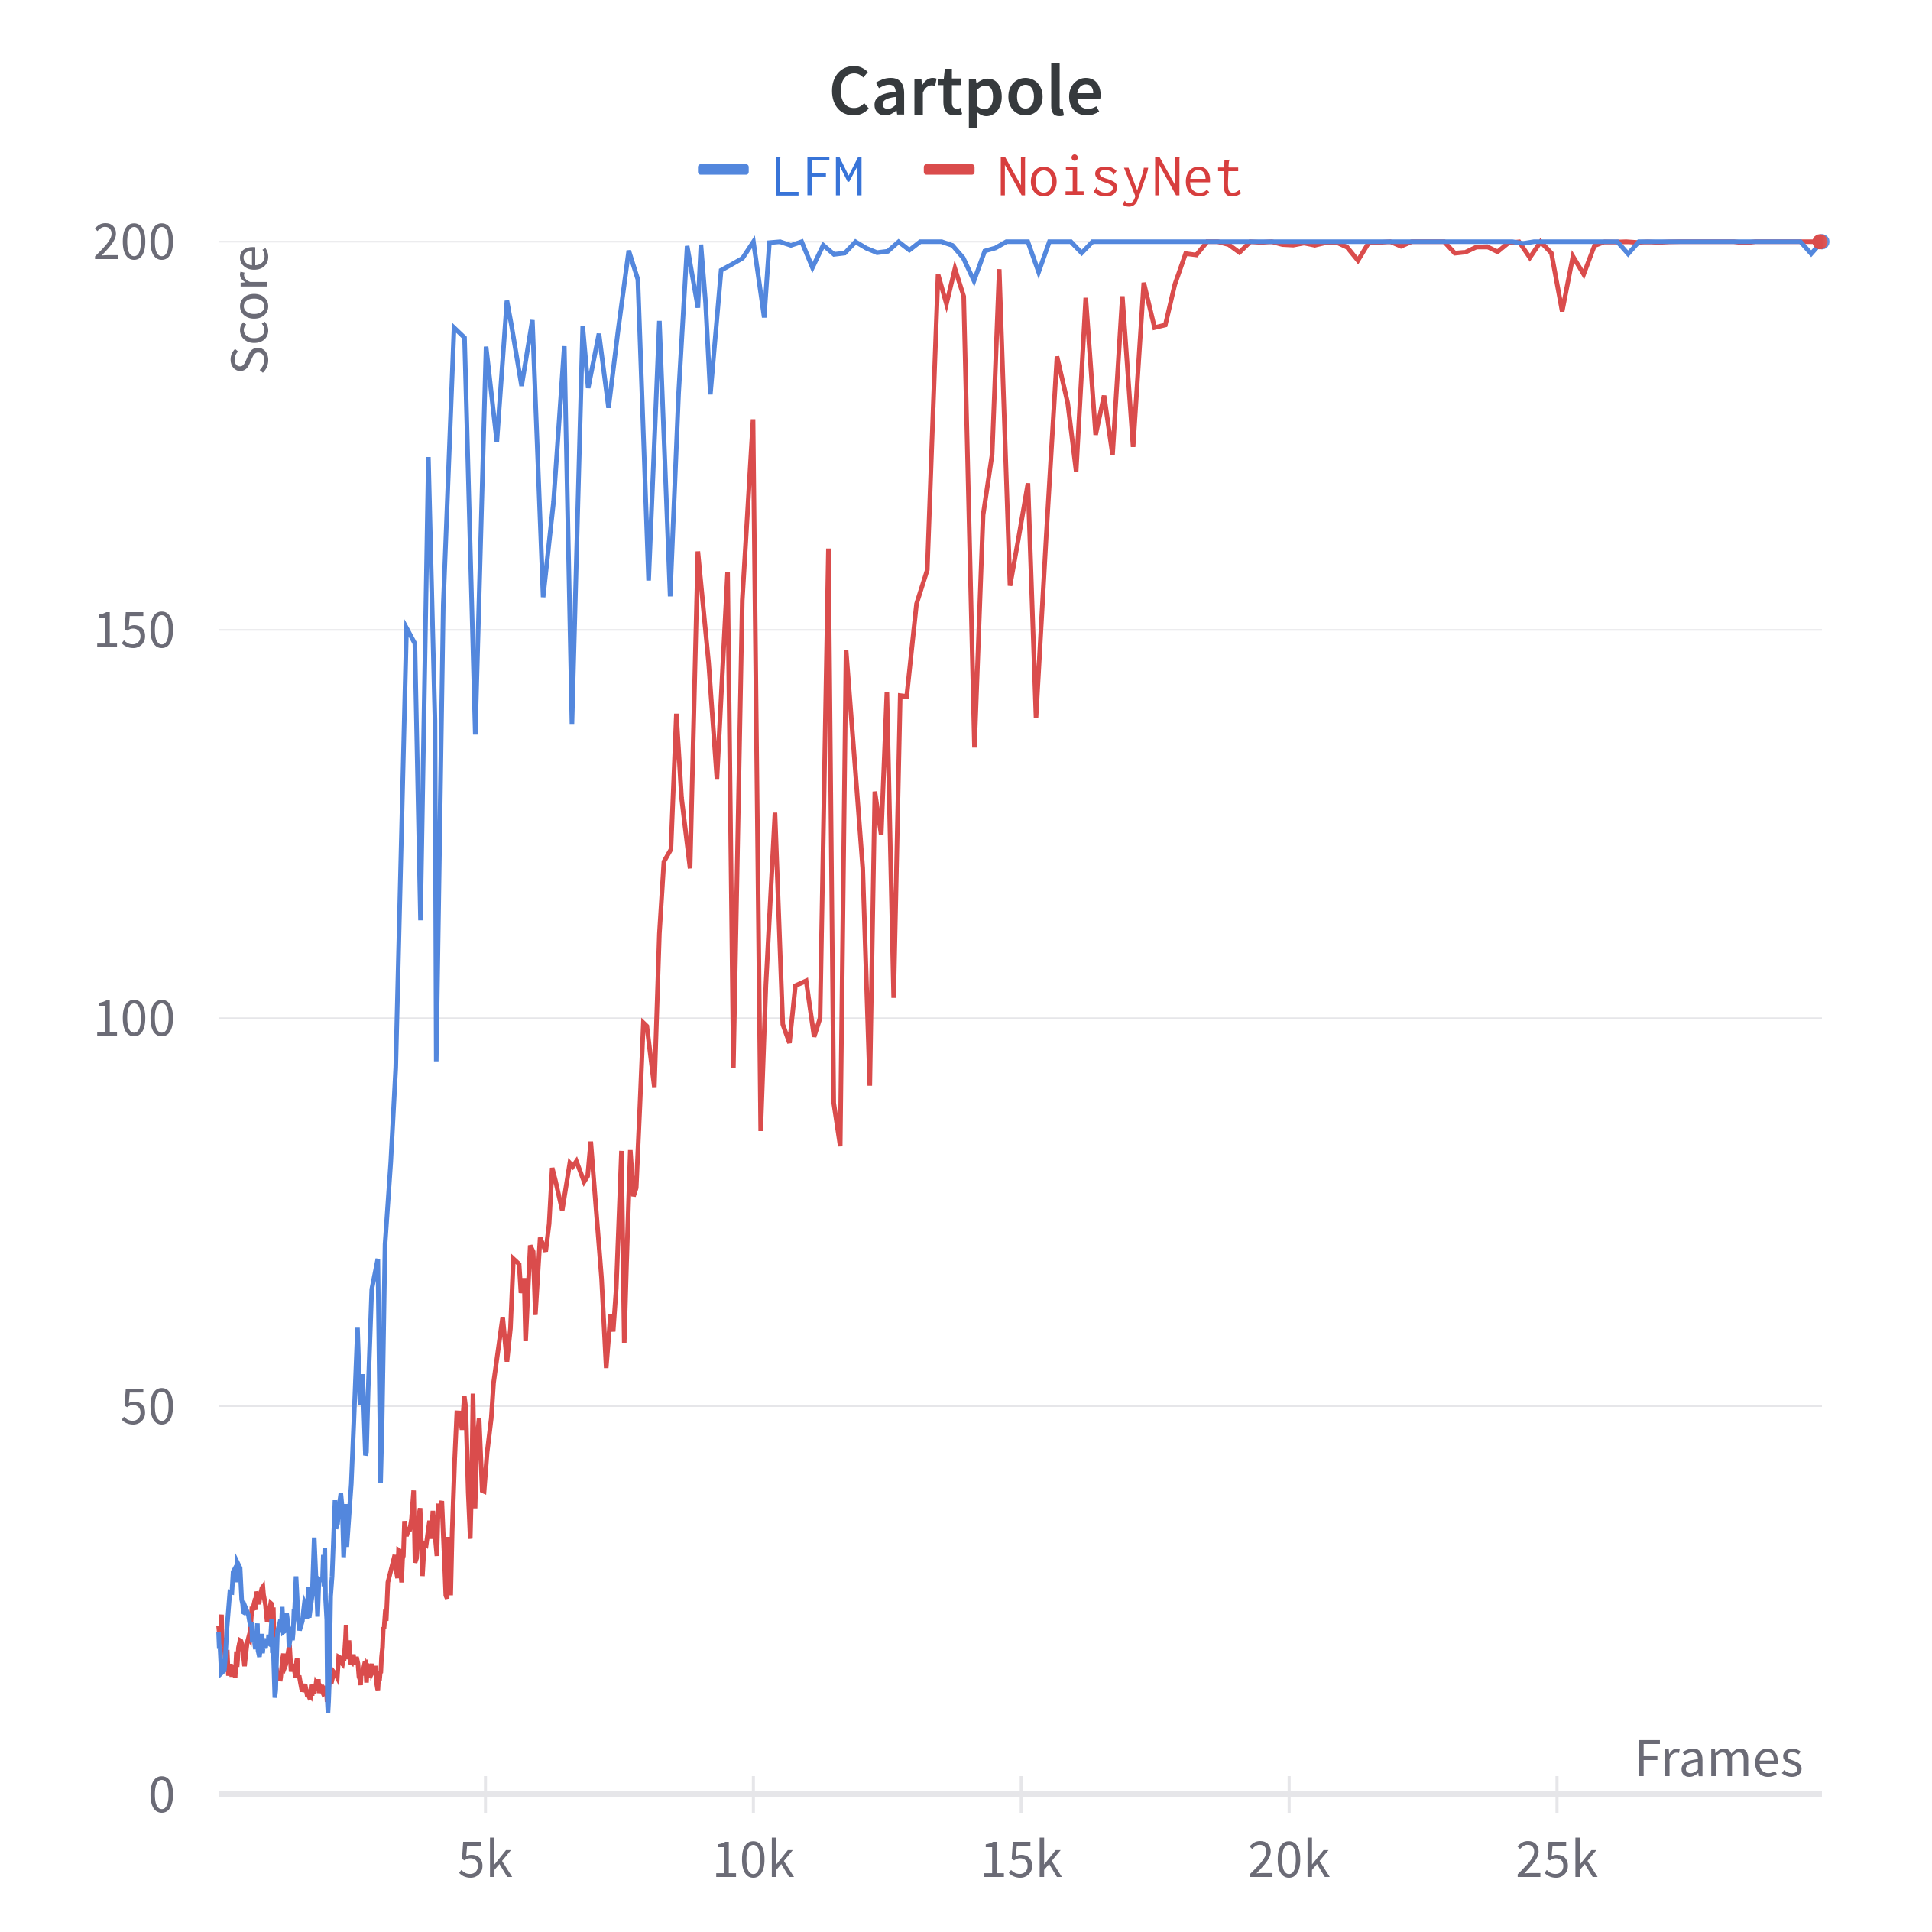
\includegraphics[width=\columnwidth]{charts/Cartpole_score}
    \end{subfigure}
    \begin{subfigure}[b]{0.45\columnwidth}
        \centering
        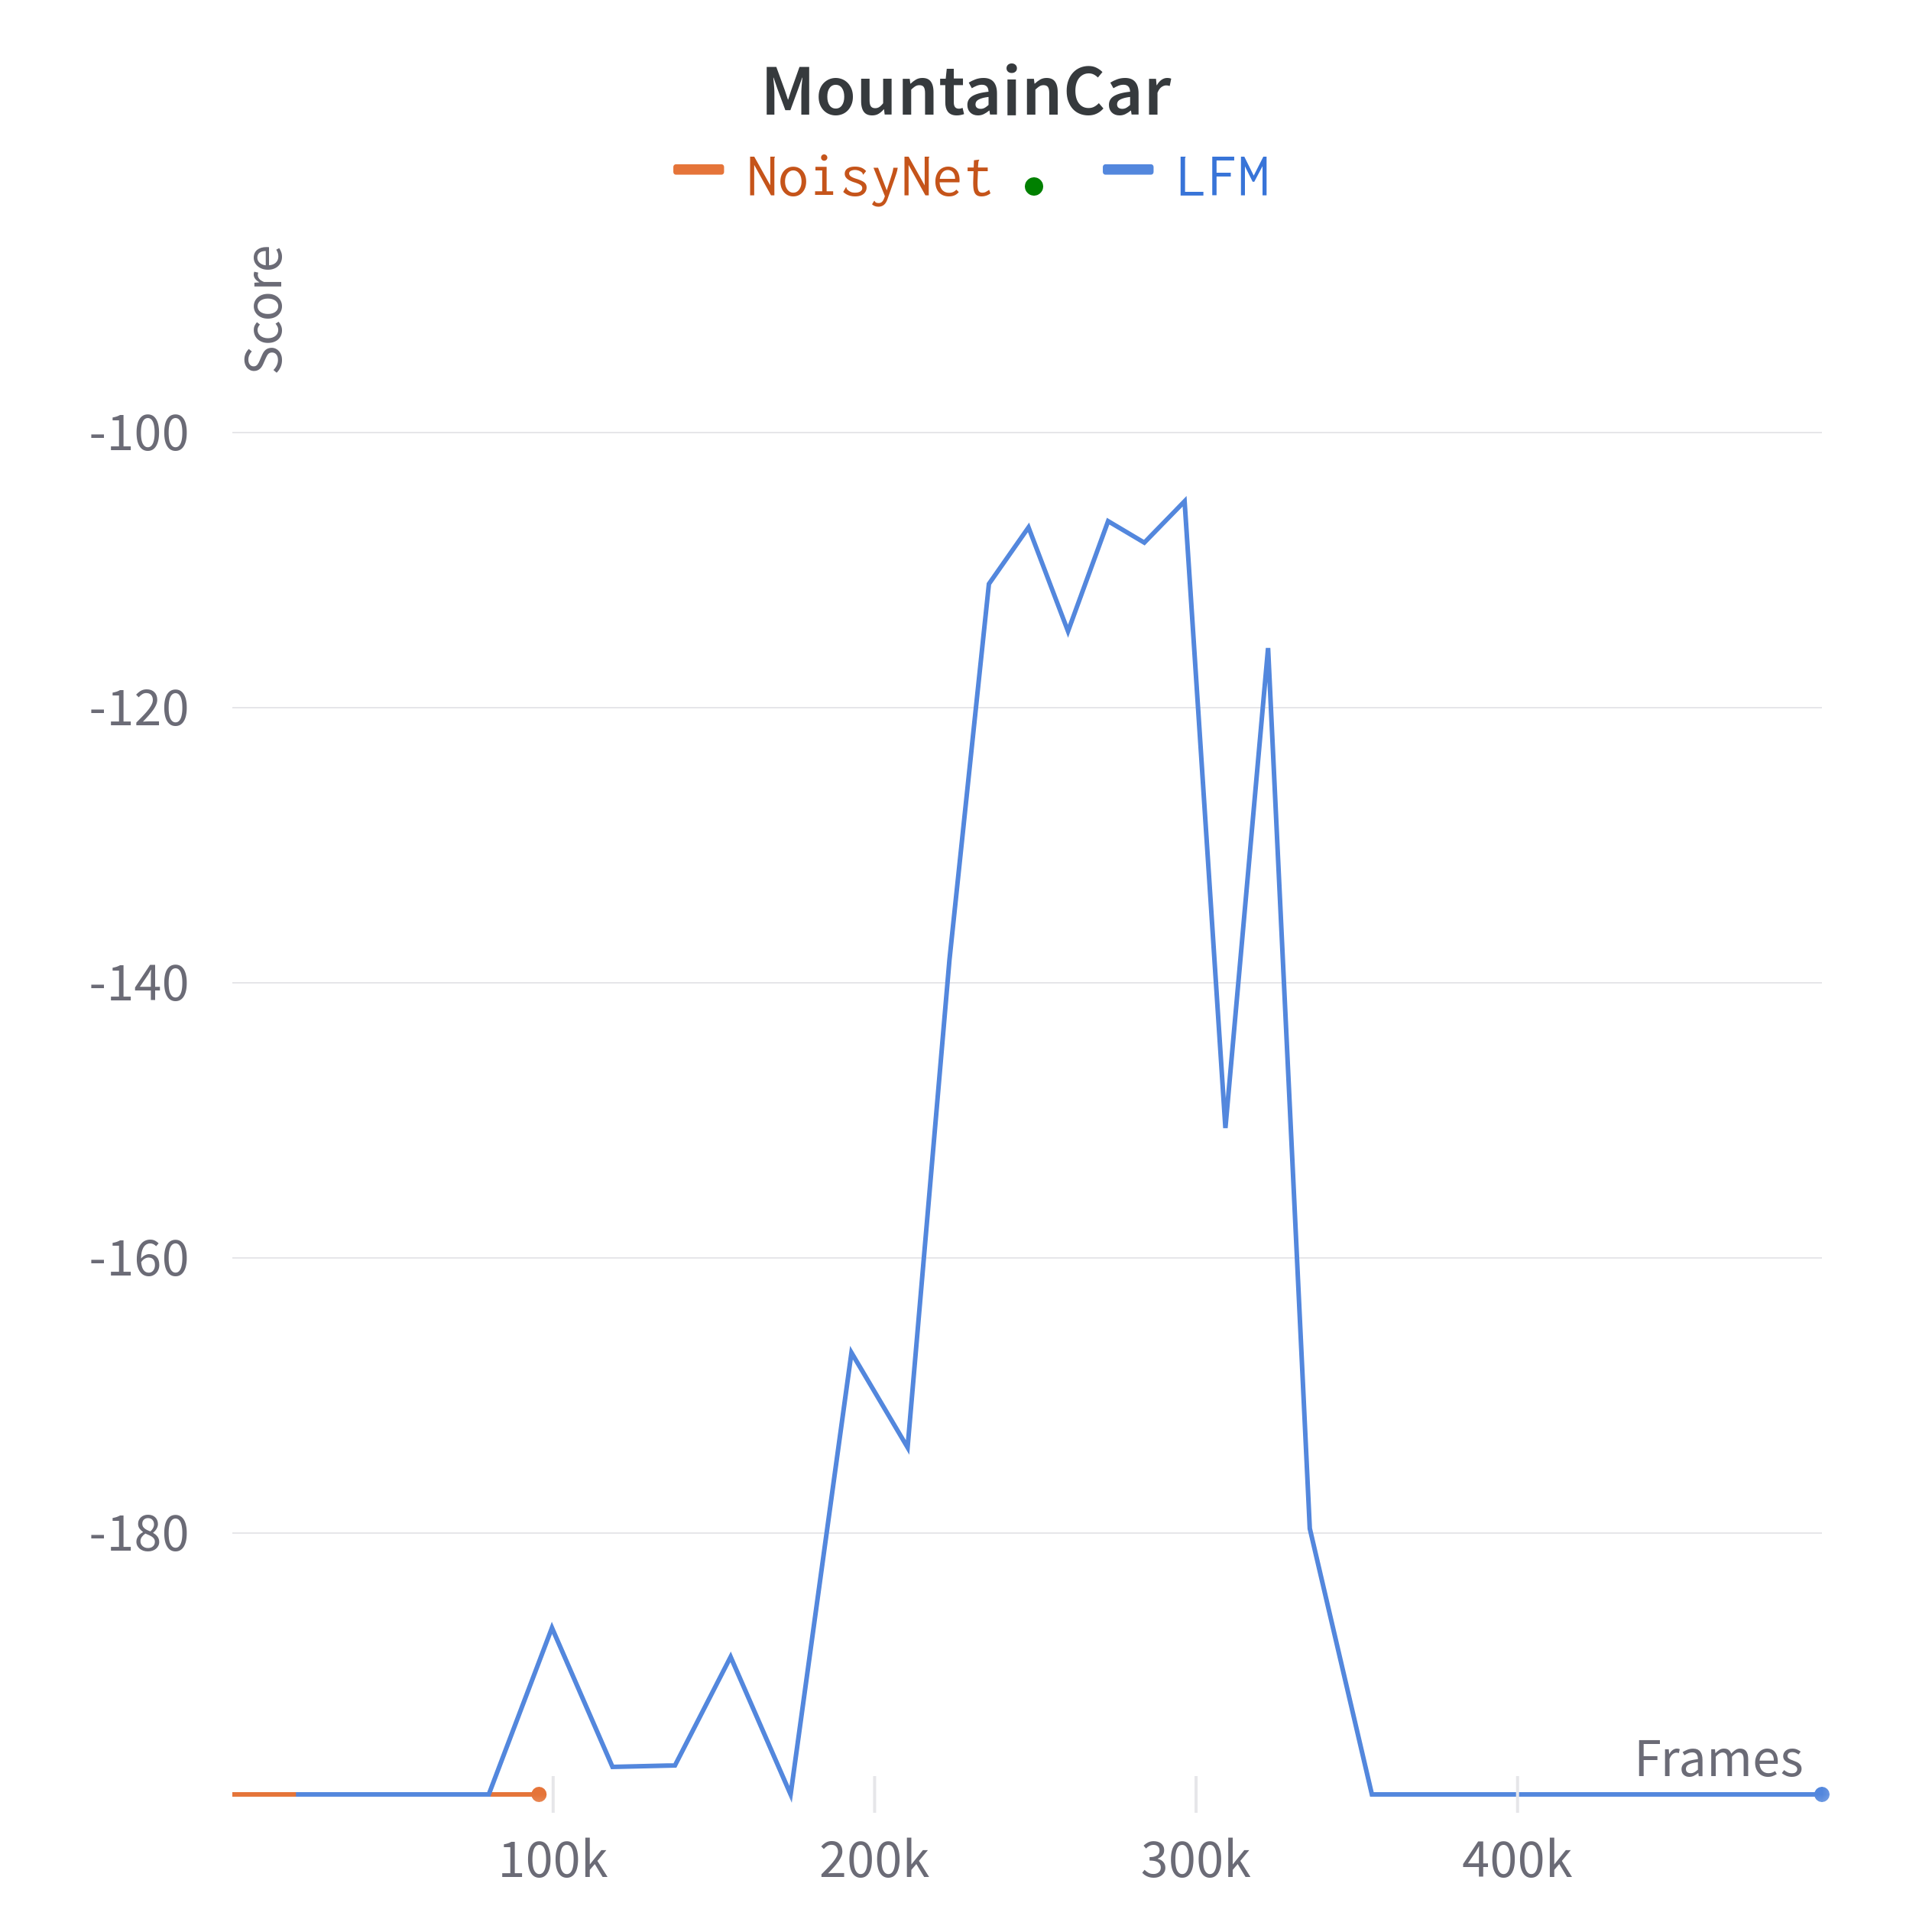
\includegraphics[width=\columnwidth]{charts/MountainCar_score}
    \end{subfigure}
    \begin{subfigure}[b]{0.45\columnwidth}
        \centering
        \includegraphics[width=\columnwidth]{example-image}
    \end{subfigure}
    \begin{subfigure}[b]{0.45\columnwidth}
        \centering
        \includegraphics[width=\columnwidth]{example-image}
    \end{subfigure}
    \caption{Comparison of learning curves of LFM and NoisyNet-DQN on
    Pong, Cartpole, MountainCar, and Acrobot averaged over 100 episodes.}
    \label{fig:training_curves}
\end{figure}

\cite{fortunato_noisy_2019} noted that the learned variance in their weight increased
in some games despite there existing an optimal deterministic solution, and the loss
provides no incentive to maintain any uncertainty. Figure~\ref{fig:mean_std} shows
the mean-absolute standard deviation for the penultimate and final layer. It is 
interesting to see that the standard deviation for NoisyNet continues to decrease
throughout the training while LFM decreases faster, but then flattens out earlier.
This seems to indicate that it has found a stable policy, where optimizing further would
be overfitting to noise.

\begin{figure}
    \centering
    \begin{subfigure}[b]{0.45\columnwidth}
        \centering
        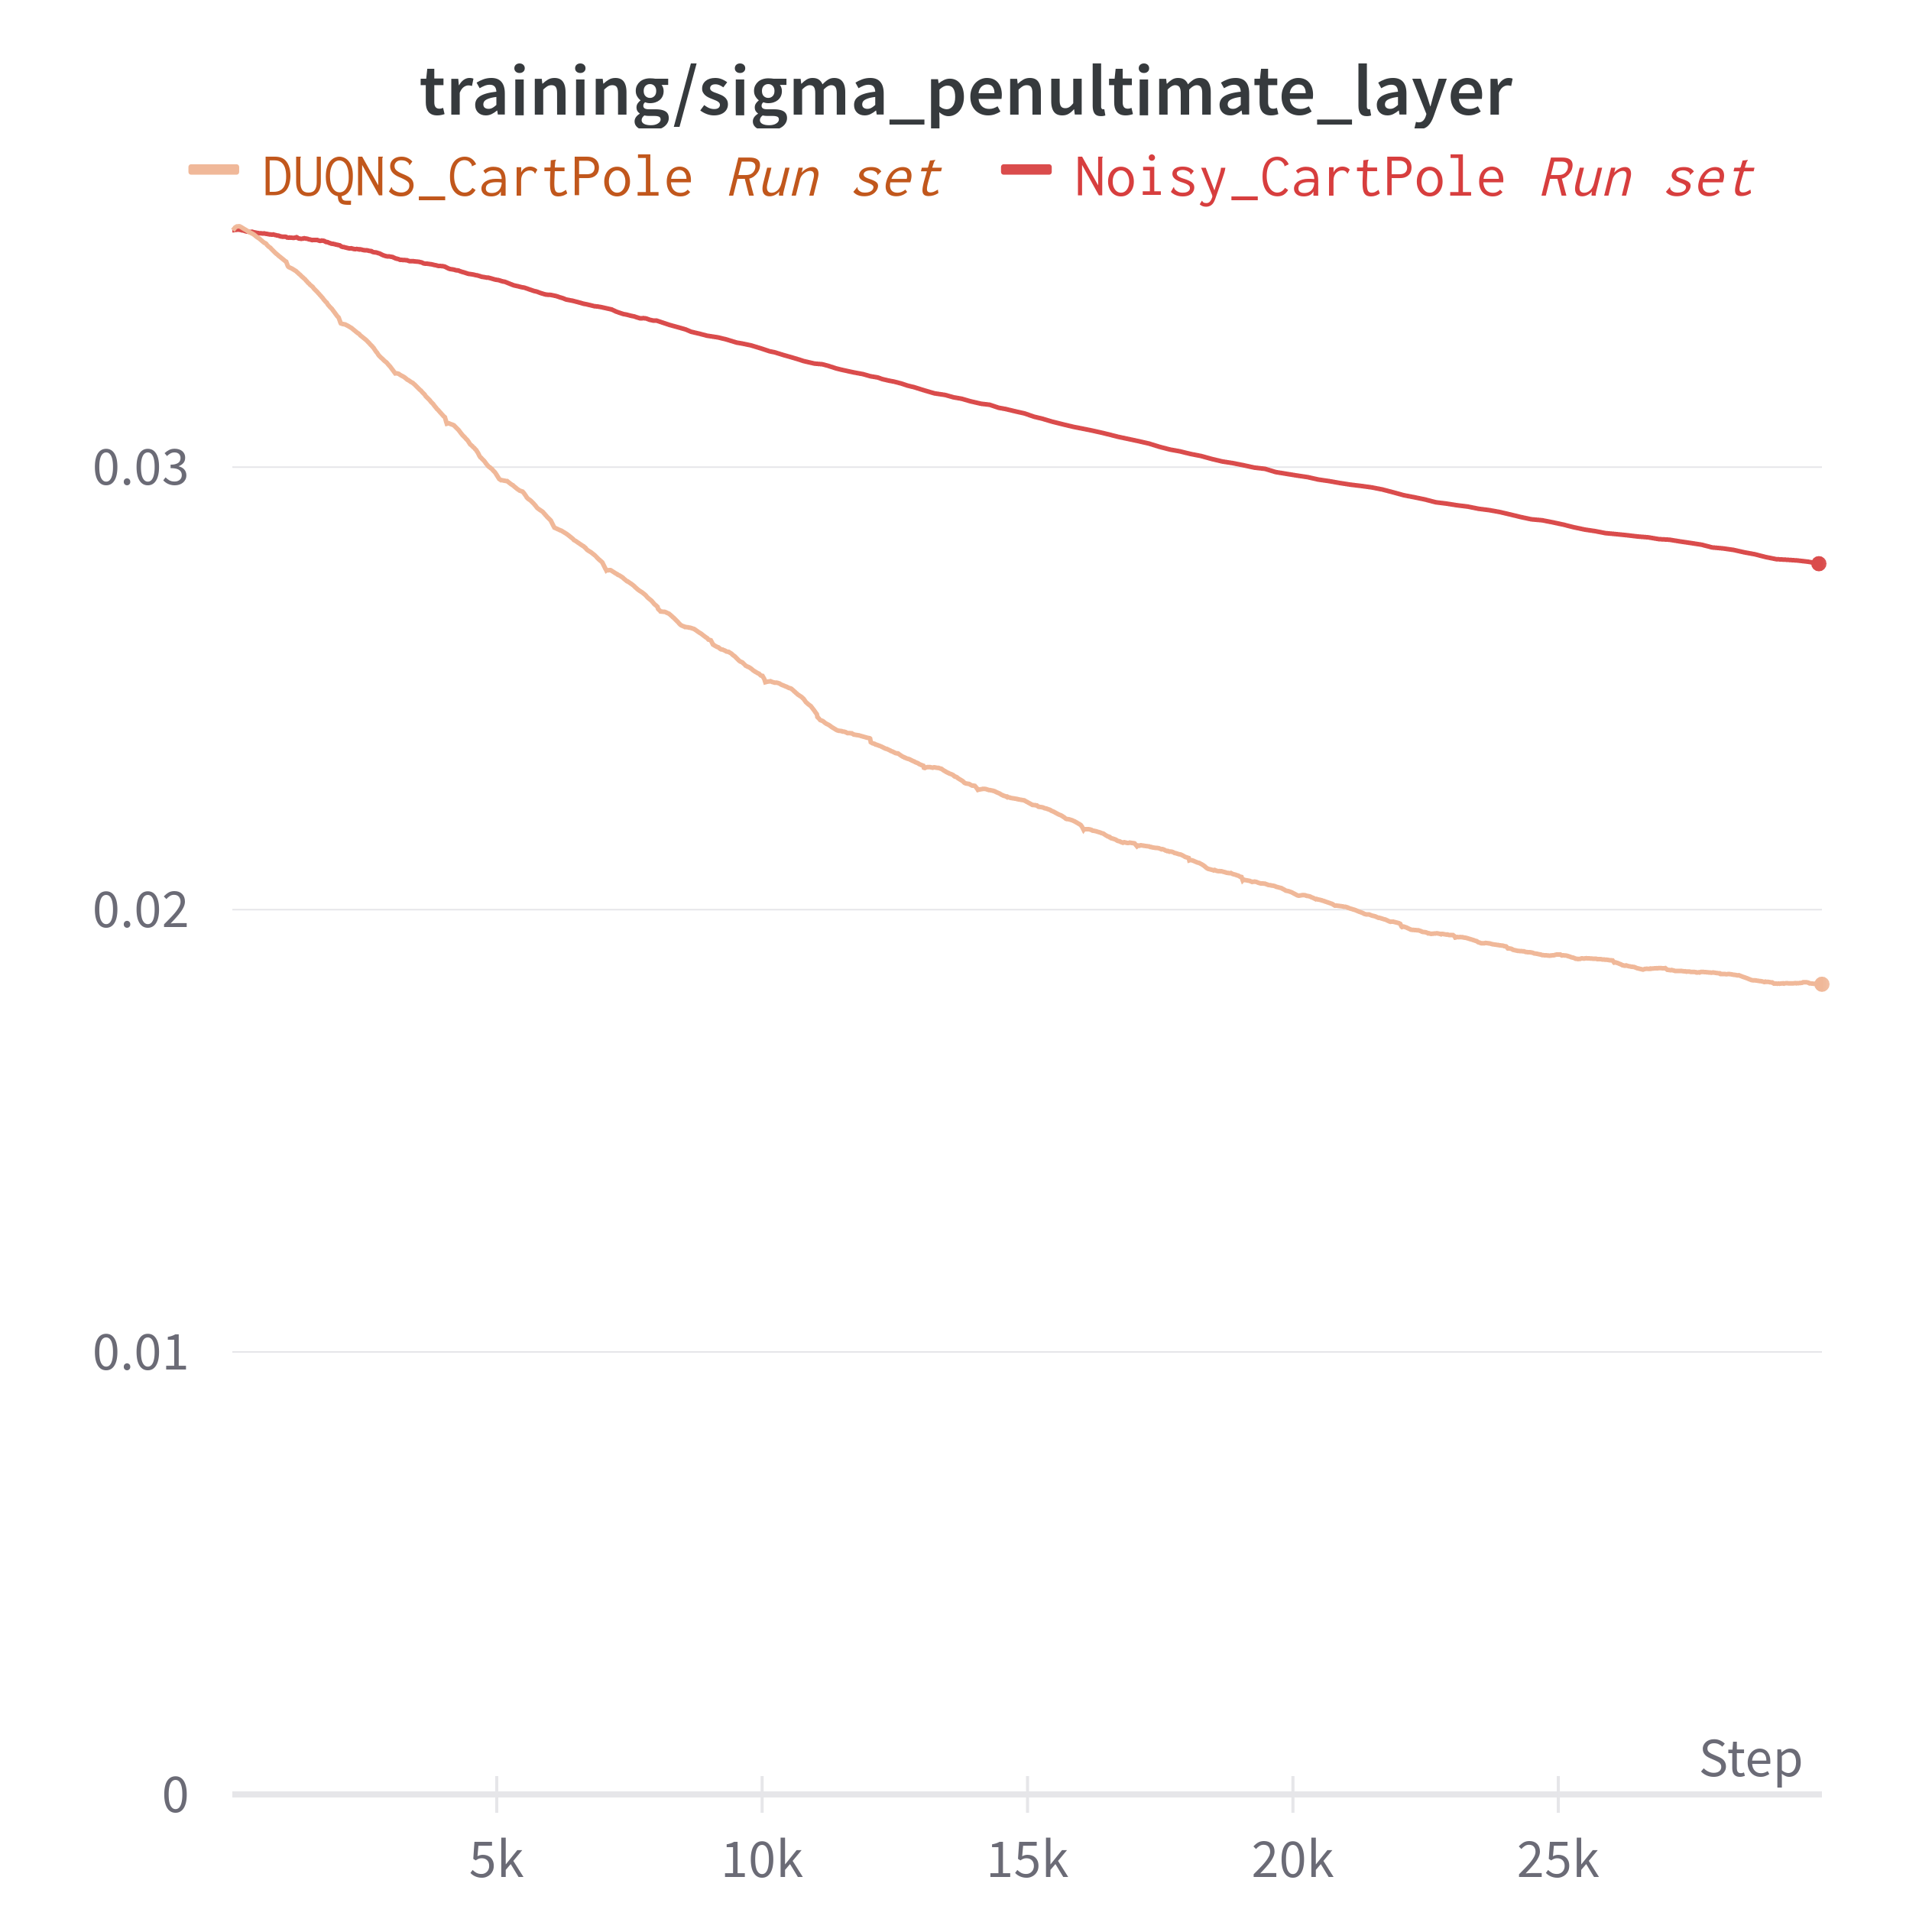
\includegraphics[width=\columnwidth]{charts/penult}
    \end{subfigure}
    \begin{subfigure}[b]{0.45\columnwidth}
        \centering
        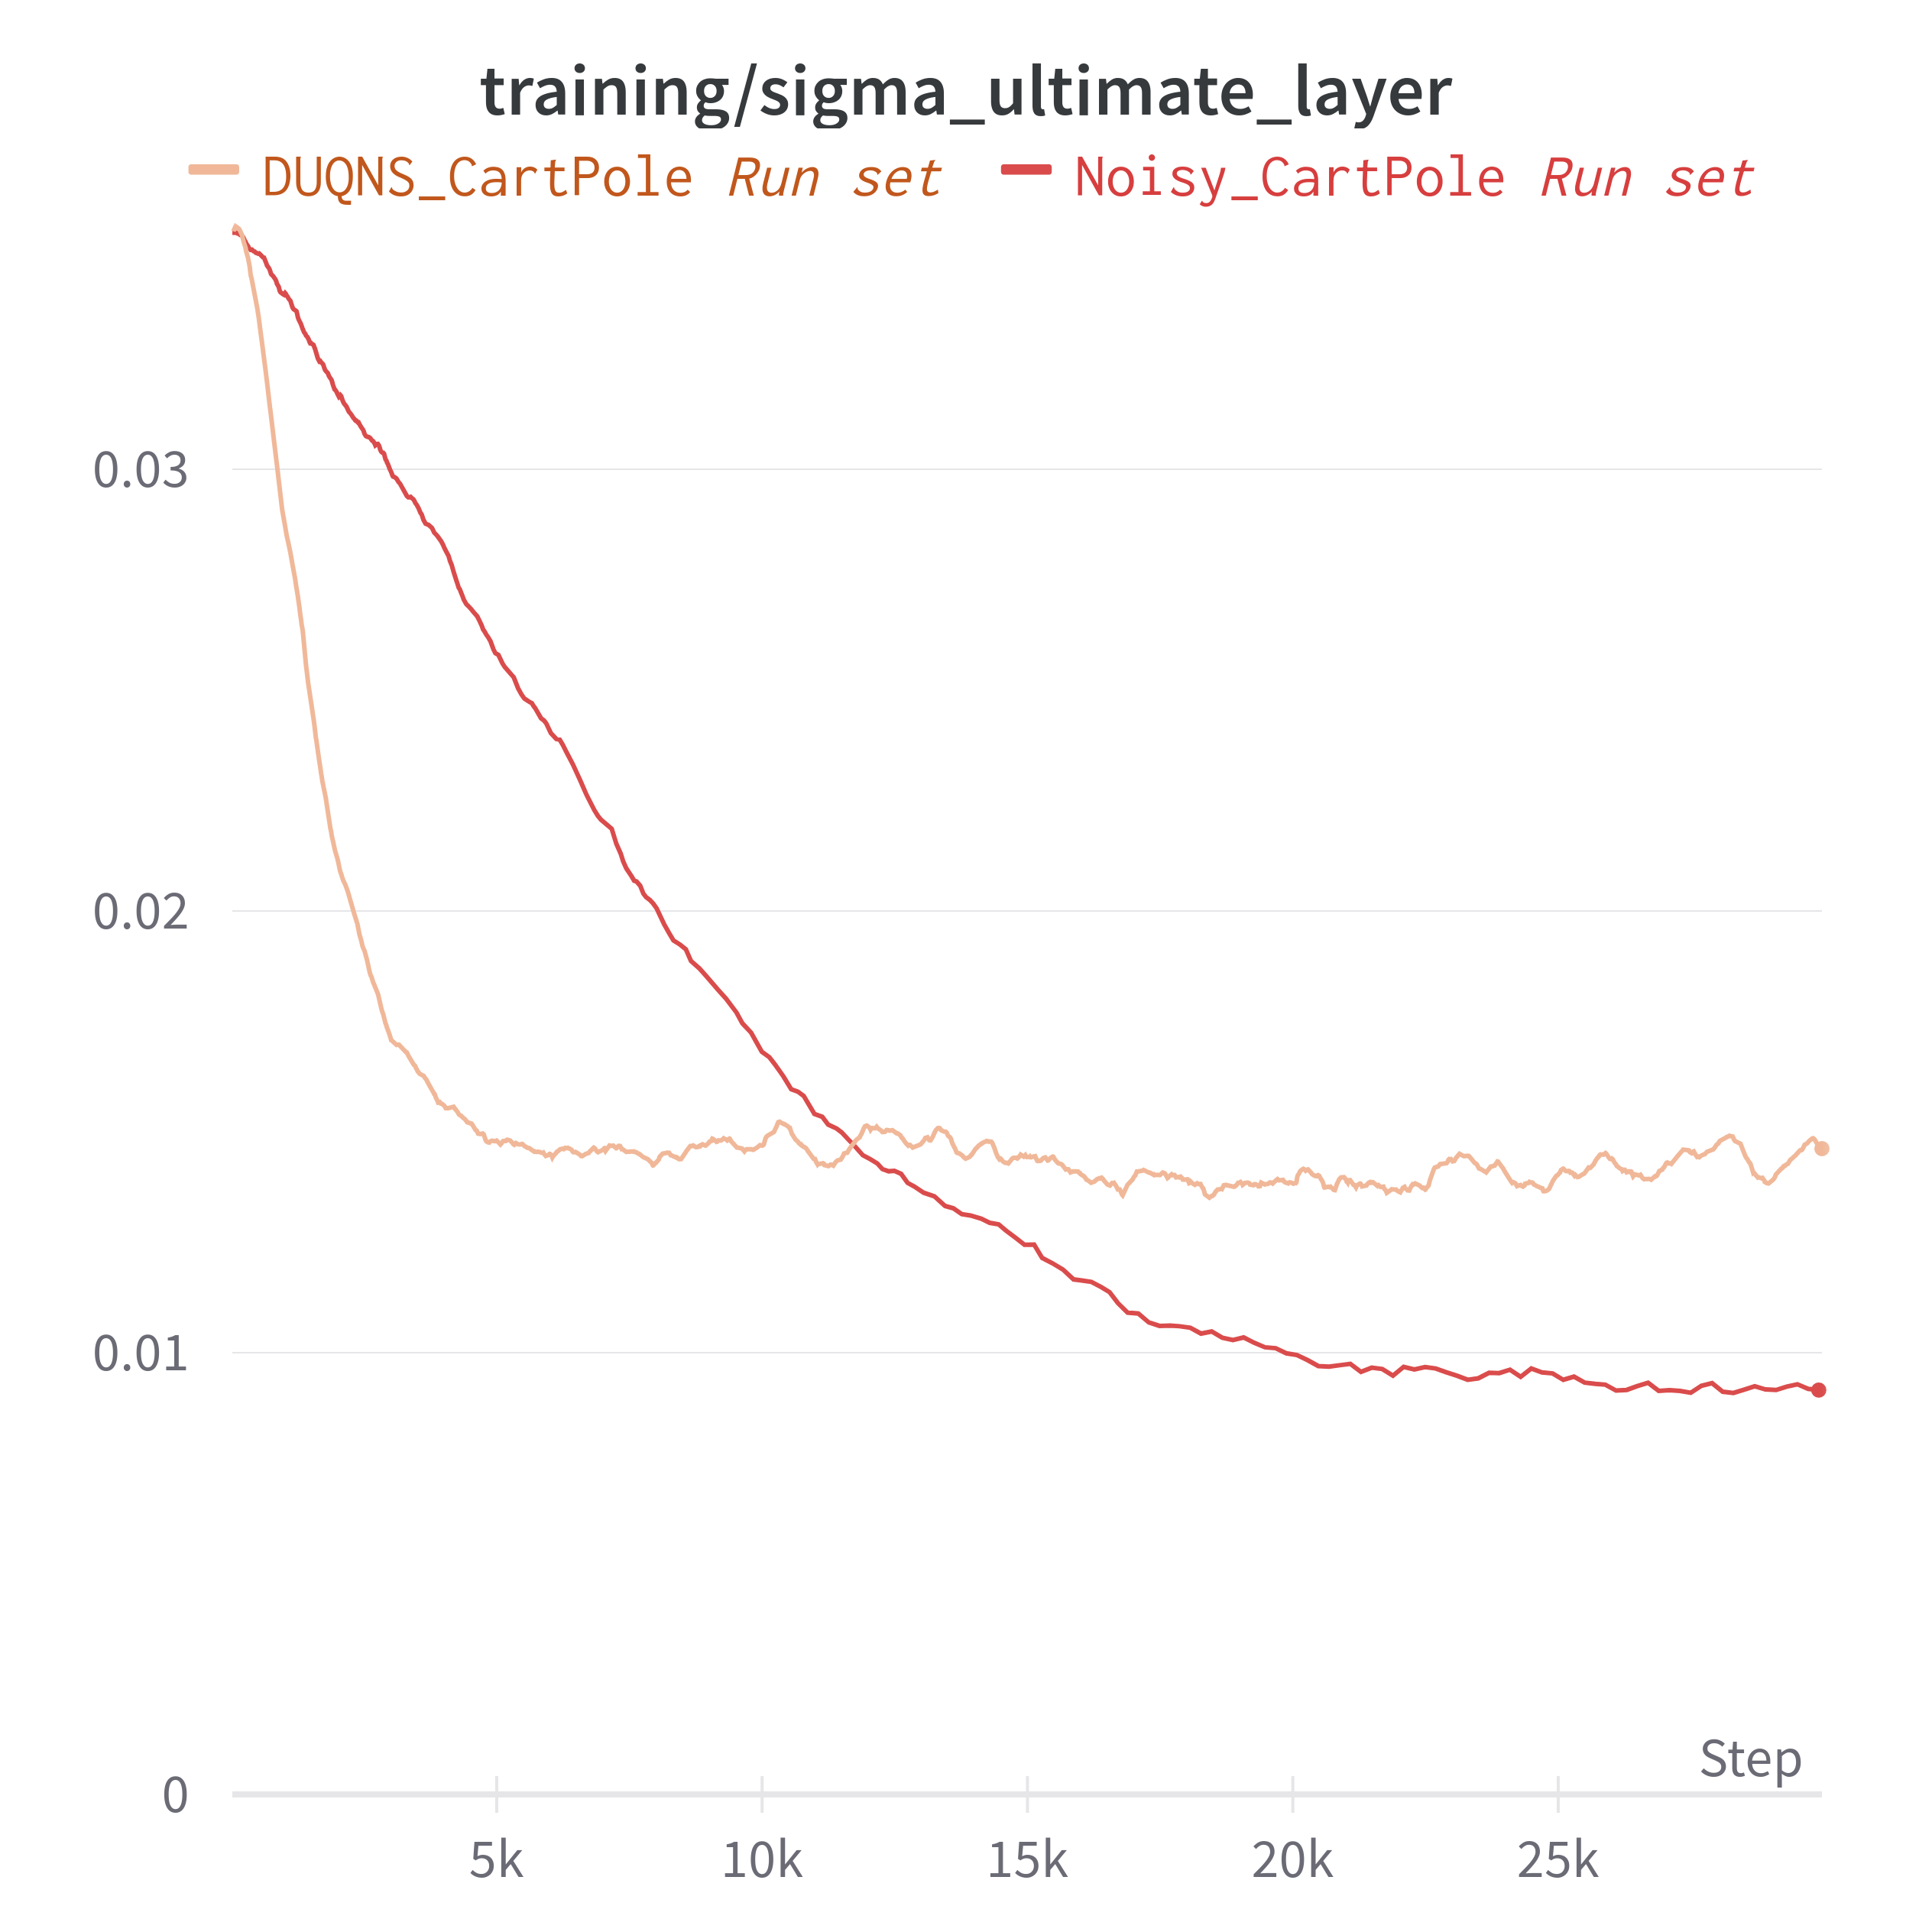
\includegraphics[width=\columnwidth]{charts/ult}
    \end{subfigure}
    \caption{Comparison of mean-absolution standard deviation for NoisyNet and LFM
    on Cartpole.}
    \label{fig:mean_std}
\end{figure}

\subsection{Informative Prior}
One of the benefits of a functional prior is that we can incorporate domain knowledge to
get more efficient exploration. We will now look at how our method can utilize domain
knowledge to improve sample efficiency.

% We will use the following method to calculate the prior distribution on the Q-values:

% \textcolor{red}{Discuss how to go from policy prior to Q-value prior.}

% \begin{figure}
%     \centering
%     \begin{subfigure}[b]{0.45\columnwidth}
%         \centering
%         \includegraphics[width=\columnwidth]{example-image}
%     \end{subfigure}
%     \begin{subfigure}[b]{0.45\columnwidth}
%         \centering
%         \includegraphics[width=\columnwidth]{example-image}
%     \end{subfigure}
%     \includegraphics[width=\columnwidth]{example-image}
%     \caption{Performance on the CartPole-v1 environment.}
% \end{figure}


\section{Conclusion and Discussion}
We have presented a method for exploration with a DQN-style algorithm that can
effectively utilize domain knowledge for faster learning. Our results show that
it outperforms standard DQN with NoisyNet exploration with regards to sample efficiency
on all four selected environments even without prior knowledge.

One interesting avenue for future work is to extend the approach to methods other than
the standard DQN. A functional Bayesian approach for policy evaluation would permit direct
prior distribution in policy space rather than in value space, which seems like a
more intuitive prior in many domains.


\begin{acknowledgements} % will be removed in pdf for initial submission,
                         % so you can already fill it to test with the
                         % ‘accepted’ class option
    Briefly acknowledge people and organizations here.

    \emph{All} acknowledgements go in this section.
\end{acknowledgements}

\bibliography{uai2021-template}

\appendix
% NOTE: necessary when ptmx or no mathfont class option is given
% \providecommand{\upGamma}{\Gamma}
% \providecommand{\uppi}{\pi}
% \section{Math font exposition}
% How math looks in equations is important:
% \begin{equation*}
%   F_{\alpha,\beta}^\eta(z) = \upGamma(\tfrac{3}{2}) \prod_{\ell=1}^\infty\eta \frac{z^\ell}{\ell} + \frac{1}{2\uppi}\int_{-\infty}^z\alpha \sum_{k=1}^\infty x^{\beta k}\mathrm{d}x.
% \end{equation*}
% However, one should not ignore how well math mixes with text:
% The frobble function \(f\) transforms zabbies \(z\) into yannies \(y\).
% It is a polynomial \(f(z)=\alpha z + \beta z^2\), where \(-n<\alpha<\beta/n\leq\gamma\), with \(\gamma\) a positive real number.

\end{document}
